\scanpage{148}

et \unsure{ses|les} accouplements \deleted{\unsure{déduisent} du \unsure{isomorphisme}}
\[
\mathbb{R}\mathcal{H}om^\bullet(L_\bullet,M_\bullet)\times\mathbb{R}\mathcal{H}om(M_\bullet,L_\bullet)\unsure{\text{---}|\longrightarrow}A_X
\]
\unsure{identifient} chacun des deux \unsure{facteurs} $P_\bullet,Q_\bullet$ du premier membre au ``dual'' de l'autre
\[
P_\bullet\simeq\mathbb{R}\mathcal{H}om(Q_\bullet,A_X),\quad Q_\bullet\simeq\mathbb{R}\mathcal{H}om(P_\bullet,A_X^{\unsure{\bullet}}).
\]

Du point de vue \unsure{cohomos}, si $u^{(i)}:L_\bullet\unsure{\text{---}|\longrightarrow}M_\bullet[i]$;
$v^{(-i)}:M_\bullet\longrightarrow L_\bullet[-i]$, \unsure{donc}
\deleted{$\unsure{L_\bullet\longrightarrow L_\bullet}$}
$v^{(-i)}u^{(i)}:L_\bullet\longrightarrow M_\bullet$.
et
\[
\langle u^{(i)},v^{(-i)}\rangle=\sum\operatorname{Tr}(uv)_{\unsure{i}}^{\unsure{i}}(-1)^{\unsure{i}}.
\]

\figure{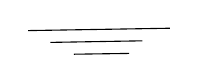
\begin{tikzpicture}[x=1cm,y=1cm]
\draw (0,0)--(1.8,.03);\draw (.28,-.15)--(1.45,-.13);\draw (.58,-.3)--(1.28,-.29);
\end{tikzpicture}}
\margin{\textcircled{c}}
Dans le cas \unsure{2)}, \inserted{$f$ et $g$ propres,} supposons que $S$ est discret,
\deleted{\unsure{bornés}}
\inserted{$F_\bullet,G_\bullet$ à \unsure{ch.} constructibles à tor.-dim finie,}
\deleted{\unsure{par dualité}}
\unsure{donc} on trouve
que $\operatorname{Hom}^{0}(\mathbb{R}f_*(F_\bullet),\mathbb{R}g_*(G_\bullet))$ et
$\operatorname{Hom}^{0}(\mathbb{R}g_*(G_\bullet),\mathbb{R}f_*(F_\bullet))$
\inserted{ou $\mathbb{R}\mathcal{H}om^\bullet(-,\cdot)$ et $\mathbb{R}\mathcal{H}om^\bullet(\cdot,-)$ \unsure{les}}
sont duaux l'un de l'autre; je dis que cette dualité est \uline{induite par un accouplement}
\diagram{\fbox{\begin{tikzcd}[ampersand replacement=\&,column sep=small]
\mathbb{R}\mathcal{H}om^\bullet(\deleted{\unsure{f^*}}\inserted{\operatorname{pr}_1^*}(F_\bullet),\operatorname{pr}_2^!(G_\bullet))\times \& \mathbb{R}\mathcal{H}om(\operatorname{pr}_2^*(G_\bullet),\operatorname{pr}_1^!(F_\bullet))\arrow[d]\\
\&K^\bullet_{X\times_S Y}=\deleted{\unsure{f}}\inserted{h}^!(A_S)
\end{tikzcd}}}
que l'on décrit ainsi (sans hyp. de propreté sur $f,g$ !) On a $Z=X\times_S Y$
\margin{147}
